\documentclass{article}

\usepackage{amsmath}
\usepackage{amssymb}
\usepackage{graphicx}
\usepackage{tikz}
\usetikzlibrary{arrows}
\usepackage{verbatim}
%\usepackage{sfmath}
\usepackage{psfrag}
\usepackage{here} 
\usepackage{hyperref}
\usepackage{xcolor}
\usepackage{tcolorbox}
\usepackage{multimedia}

%\renewcommand\sfdefault{phv}%               use helvetica for sans serif
\renewcommand{\familydefault}{\sfdefault}
\renewcommand{\familydefault}{cmss}

\setcounter{MaxMatrixCols}{60} %configuring the graphicx package
\title{Problem 1}
\author{Javier Izquierdo Hernández}
\date{\today}
\begin{document}
	\begin{titlepage}
	\centering
	{
\includegraphics[width=0.3\textwidth]{figures/logo}\par}
	\vspace{1cm}
	{\bfseries\LARGE Universidad Rey Juan Carlos \par}
	\vspace{1cm}
	{\scshape\Large E.T.S. Ingeniería de Telecomunicación \par}
	\vspace{3cm}
	{\scshape\Huge Ingeniería de Control \par}
	\vspace{3cm}
	{\itshape\Large Problem 1 \par}
	\vfill
	{\Large Autor: \par}
	{\Large Javier Izquierdo Hernández \par}
	\vfill
	{\Large \today \par}
\end{titlepage}

\begin{center}
\huge \bf Problem 1 
\footnote{Adapted from \href{https://www.ensta-bretagne.fr/jaulin/automooc.pdf}{https://www.ensta-bretagne.fr/jaulin/automooc.pdf}}
\end{center}



\tcbset{colframe=black,colback=white,colupper=black,fonttitle=\bfseries,nobeforeafter,center title}

Let us consider the car-trailer system represented in Figure~\ref{fig:figure} which has the following state equations:


\begin{eqnarray*}
\begin{pmatrix}
\dot{x}    \\       
\dot{y}      \\     
\dot{\theta} \\   
\dot{\theta}_r\\ 
\dot{v}           \\
\dot{\delta}   
\end{pmatrix}
=
\begin{pmatrix}
v \cos \delta \cos \theta \\
v \cos \delta \sin \theta\\
\frac{v \sin \delta}{L}\\
\frac{v \cos \delta \sin (\theta -\theta_r)}{L_r}\\
u_1\\
u_2
\end{pmatrix}.
\end{eqnarray*}
The state vector is given by
\begin{equation*}
\mathbf{x} 
=
\begin{pmatrix}
x\\
y\\
\theta\\
\theta_r\\
v\\
\delta
\end{pmatrix},
\end{equation*}
where $x, y, \theta$ corresponds to the pose of the car (in other words, its position and orientation), $\theta_r$ is the orientation of the trailer, $v$ is the speed and $\delta$ is the angle of the front wheels of the car. The
parameter $L = 3$ [m] is the distance between the two axles of the car.
The parameter $L_r = 5$ [m] represents the distance between the
attachment point and the middle of the axle of the trailer.

\begin{figure}[H]
\centerline{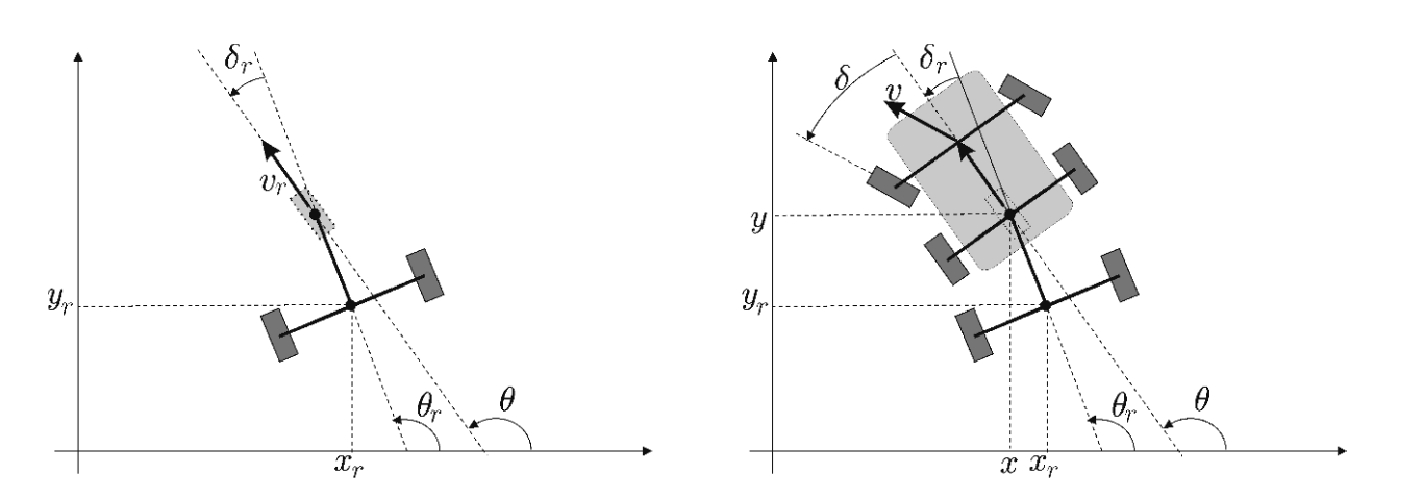
\includegraphics[width=0.99\columnwidth]{figures/car-trailer}}
\caption{The car-trailer system.}
\label{fig:figure}
\end{figure}



\begin{itemize}

\item[1)] Using homogeneous coordinates, design a function which draws a car-trailer system in a state $\mathbf{x} =
(x, y, \theta, \theta_r, v, \delta)^T$ using the sketch of the car-trailer system represented in Figure~\ref{fig:figure1} 
whose vertices in homogeneous coordinates are represented by the columns of the following matrix:
(Contesta en el informe y sube el c\'odigo \texttt{Matlab} a Aula Virtual)

\begin{scriptsize}
 \begin{equation*}
M_{\text{trailer}} =
\begin{pmatrix}
-1 & 2  &5  &5 &2 &-1 &-1 &-1 &0  &0  &-1  &1  &0 &0 &-1 &1 &0 &0 &2 \\
-2 &-2 &0  &0 &2 &2  &-2 &-2 &-2 &-3 &-3 &-3 &-3 &3  &3 &3 &3 &2 &2\\
1 &1 &1  &1   &1   &1 &1 &1 &1 &1 &1 &1 &1 &1 &1 &1 &1 &1 &1
\end{pmatrix}.
\end{equation*}
\end{scriptsize}
The corresponding \texttt{Matlab} code is:
\begin{scriptsize}
\begin{verbatim}
M_trailer=[-1  2  5  5 2 -1 -1 -1 0  0  -1  1  0 0 -1 1 0 0 2; 
           -2 -2  0  0 2 2  -2 -2 -2 -3 -3 -3 -3 3  3 3 3 2 2;
           ones(1,19)];
\end{verbatim}                    
\end{scriptsize}                    
                    
                    
\begin{figure}[H]
\centerline{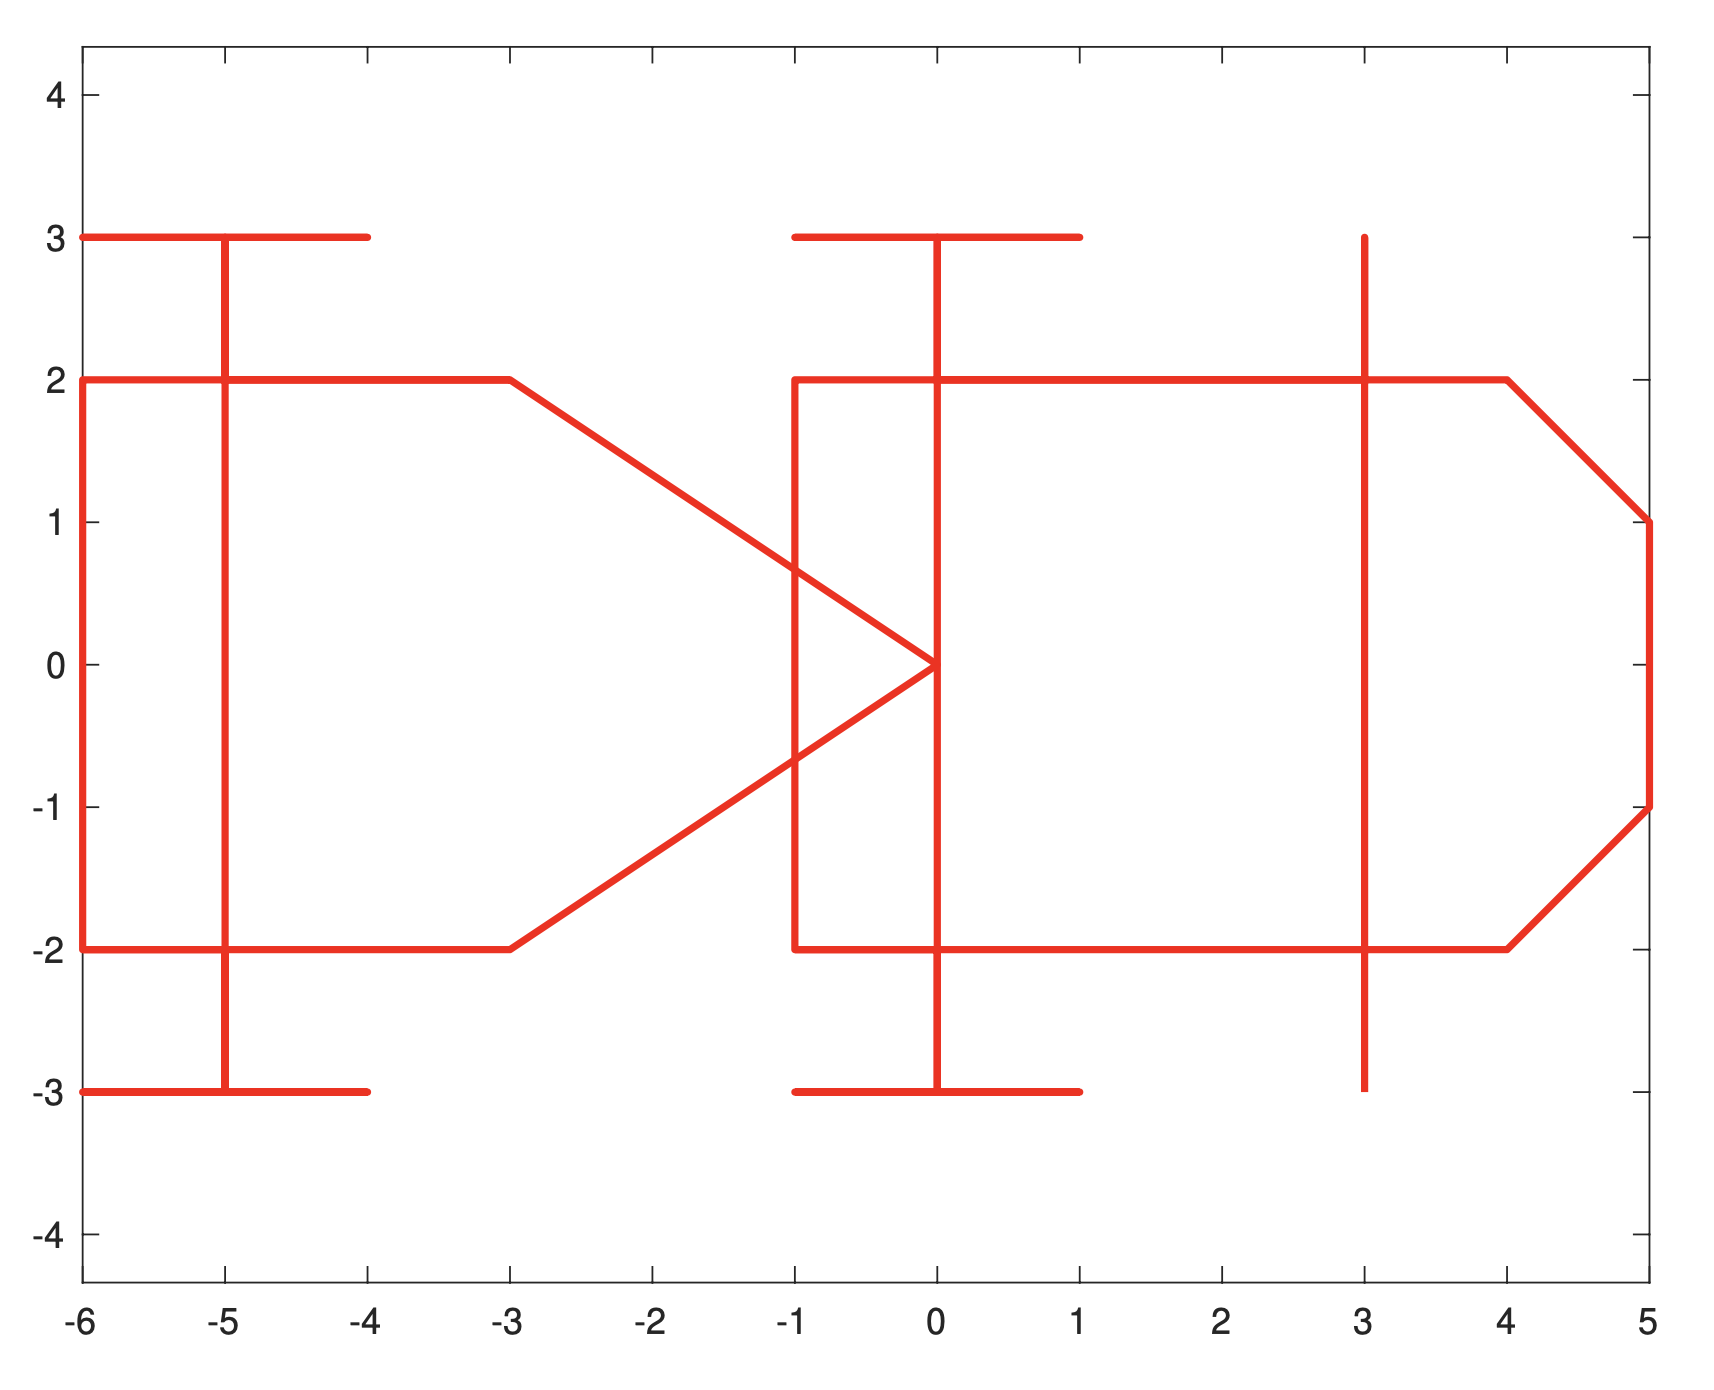
\includegraphics[width=0.99\columnwidth]{figures/chassis-trailer}}
\caption{Sketch of the car-trailer system.}
\label{fig:figure1}
\end{figure}



\item[2)] Propose a program which simulates the dynamic evolution of this car-trailer system during $5$ seconds with
Euler's method and a sampling step of $0.01 \; [\text{s}]$. Take the initial state for the car-trailer system as $\mathbf{x}(0) =
(0, 0, 0, 0, 50, 0)^T$, which means that, at time $t = 0$,

\begin{itemize}

\item
the car is centered around the origin, with a zero orientation angle, a speed of $50 \; [\text{m s}^{-1}]$ and the front wheels parallel to the axis of the car. 

\item
 the trailer has zero orientation angle. 

\end{itemize}

We assume
that the vectorial control $u(t)$ remains constant and equal to $(0, 0.05)$. Which means that the car
does not accelerate (since $u_1 = 0$) and that the steering wheel is turning at a constant speed of
$0.05 \; [\text{rad s}^{-1}]$. (Contesta en el informe y sube el c\'odigo \texttt{Matlab} a Aula Virtual)

\end{itemize}

\newpage

\section*{Report}
Un cambio importante que he tenido que hacer a la estructura del problema ha sido el cambio de nombre de los ficheros car-trailer\_main.m, car-trailer\_draw.m y car-trailer\_f.m a car\_trailer\_main.m, car\_trailer\_draw.m y car\_trailer\_f.m ya que matlab no deja poner - en los nombres de ficheros.\\
\centerline{\includegraphics*[width=0.9\textwidth]{figures/matlab_error}}\\
\newline
En cuanto al código para solucionar el problema, he usado como base el que nos dieron para el ejercicio 3.4. Primero he modificado las ecuaciones del sistema para que coincidan con las del problema añadiendo thetar para el ángulo del remolque.\\
\centerline{\includegraphics*[width=0.7\textwidth]{figures/matlab_state}}\\
\newline
Con las ecuaciones del sistema ya actualizadas lo único que falta es añadir la matriz de traslación y rotación para que el remolque sea animado correctamente.\\
\newline
La matriz de traslación, que se define como: un caso particular de transformación afín pero no una transformación lineal, generalmente se usan coordenadas homogéneas para representar la traslación mediante una matriz y poder así expresarla como una transformación lineal sobre un espacio de dimensión superior. Como el eje z esta fijo $p_z$ será 1\\
\begin{scriptsize}
	\begin{equation*}
		M_{\text{tras}} =
		\begin{pmatrix}
			1 & 0  &p_x\\
			0 &1 &p_y\\
			0 &0 &1
		\end{pmatrix}.
	\end{equation*}
\end{scriptsize}
\newline
En este caso la posición del trailer viene definida por la posición central del coche, definida por $p_x$ y $p_y$, el ángulo del trailer $\theta_r$ y la distancia entre el punto enganche del trailer al coche y el centro del eje del trailer, que es 5 en este problema. Luego la matriz de traslación es:\\
\begin{scriptsize}
	\begin{equation*}
		M_{\text{tras trailer}} =
		\begin{pmatrix}
			1 & 0  &p_x - 5·cos(\theta_r) \\
			0 &1 &p_y - 5·sin(\theta_r)\\
			0 &0 &1
		\end{pmatrix}.
	\end{equation*}
\end{scriptsize}
\newline
La matriz de rotación, que se define como: la matriz que representa una rotación en el espacio euclídeo. Por ejemplo, la matriz
\begin{scriptsize}
	\begin{equation*}
		M_{\text{rot}} =
		\begin{pmatrix}
				cos(\theta) & -sin(\theta)\\
				sin(\theta) &cos(\theta)\\
		\end{pmatrix}.
	\end{equation*}
\end{scriptsize}
representa la rotación de $\theta$ grados del plano en sentido antihorario. En el caso que tenemos presente, la matriz de rotación será en 3 dimensiones, y al estar el eje z fijo la matriz de rotación respecto a $\theta$ es:
\begin{scriptsize}
	\begin{equation*}
		M_{\text{$rot_z$}} =
		\begin{pmatrix}
			cos(\theta) & -sin(\theta)  &0 \\
			sin(\theta) &cos(\theta) &0\\
			0 &0 &1
		\end{pmatrix}.
	\end{equation*}
\end{scriptsize}
\newline
En este caso la rotación del trailer viene definida por el ángulo del trailer $\theta_r$. Luego la matriz de rotación es:\\
\begin{scriptsize}
	\begin{equation*}
		M_{\text{rot trailer}} =
		\begin{pmatrix}
			cos(\theta_r) & -sin(\theta_r)  &0\\
			sin(\theta_r) &cos(\theta_r) &0\\
			0 &0 &1
		\end{pmatrix}.
	\end{equation*}
\end{scriptsize}
\newline
Luego al multiplicar la matriz de traslación y rotación conseguimos la matriz que se necesita para dibujar correctamente el trailer:
\begin{scriptsize}
	\begin{equation*}
		M_{\text{rot trailer}} =
		\begin{pmatrix}
			cos(\theta_r) & -sin(\theta_r)  &p_x - 5·cos(\theta_r) \\
			sin(\theta_r) &cos(\theta_r) &p_y - 5·sin(\theta_r)\\
			0 &0 &1
		\end{pmatrix}.
	\end{equation*}
\end{scriptsize}
\newline
El resultado final con la simulación es, si no se ve el video está disponible en  figures/video:\\
\movie[width=0.8\textwidth, height=0.8\textwidth]{Click para ver video. Se necesita visor de Pdf como Okular}{figures/video.mp4}
\newpage

\section*{Solution}


\noindent
    \begin{tcolorbox}[
        title={File \texttt{init.m}},
%        halign=center,
%        valign=center,
%        nobeforeafter,
        width=13cm,
    ]
    
\begin{scriptsize}
\begin{verbatim}

close all; 
clear all; 
clc;

figure
hold

xmin=-10;
xmax=100;
ymin=-10;
ymax=100;

axis([xmin xmax ymin ymax]); 
axis ('square');

\end{verbatim}
\end{scriptsize}
\end{tcolorbox}










\bigskip

\noindent
    \begin{tcolorbox}[
        title={File \texttt{car\_trailer\_f.m}},
%        halign=center,
%        valign=center,
%        nobeforeafter,
        width=13cm,
    ]
    
\begin{scriptsize}
\begin{verbatim}

function  xdot  = f(x,u)
% state x = (x,y,theta,thetar,v,delta)
% control u=(u1 u2)
L=3;
Lr=5;

px=x(1);
py=x(2);
theta=x(3);
thetar=x(4);
v=x(5);
delta=x(6);

xdot=[v*cos(delta)*cos(theta); v*cos(delta)*sin(theta);v*sin(delta)/L;
(v*cos(delta)*sin(theta-thetar))/Lr; u(1); u(2)];
end

\end{verbatim}
\end{scriptsize}
\end{tcolorbox}









\bigskip


\noindent
    \begin{tcolorbox}[
        title={File \texttt{car\_trailer\_draw.m}},
%        halign=center,
%        valign=center,
%        nobeforeafter,
        width=13cm,
    ]
    
\begin{scriptsize}
\begin{verbatim}

% For this system, the state is x =(x,y,theta,thetar,v,delta)
% The v state variable, since it is a speed, it is not used in this 
% graphical representation

function car_trailer_draw(x)

% Extraction of the state variables
px=x(1);
py=x(2);
theta=x(3);
thetar=x(4);
v=x(5);
delta=x(6);

% Model of the chassis of the car without front wheels (in homogeneous coordinates)
M_chassis=[-1  4 5  5 4 -1 -1 -1 0  0  -1  1  0 0 -1 1 0 0 3 3 3; 
-2 -2 -1 1 2 2  -2 -2 -2 -3 -3 -3 -3 3  3 3 3 2 2 3 -3;
ones(1,21)];

% Model of the chassis of the trailer (in homogeneous coordinates)
M_trailer=[-1 2 5 5 2 -1 -1 -1 0 0 -1 1 0 0 -1 1 0 0 2;
-2 -2 0 0 2 2 -2 -2 -2 -3 -3 -3 -3 3 3 3 3 2 2;
ones(1,19)];

% Model of a front wheel (in homogeneous coordinates)
M_wheel=[-1 1;
0 0;
1 1]; 

% Translation and rotation of the whole car (chassis and front wheels) 
% with respect to the fixed frame
TR_px_py_theta=[cos(theta),-sin(theta), px;
sin(theta),cos(theta), py;
0 0 1]; 

% Translation and rotation of the trailer with respect to the fixed frame
TR_px_py_thetar=[cos(thetar),-sin(thetar), px - 5*cos(thetar);
sin(thetar),cos(thetar), py - 5*sin(thetar);
0 0 1];

% Chassis of the car translated and rotated
M_chassis_transformed=TR_px_py_theta*M_chassis;   

% Chassis of the car translated and rotated
M_trailer_transformed=TR_px_py_thetar*M_trailer; 

% Translation and rotation matrix for the right wheel with respect to the chassis frame 
TR_right_wheel_delta = [cos(delta),-sin(delta), 3;
sin(delta),cos(delta), 3 ;
0 0 1]; 

% Translation and rotation matrix for the left wheel with respect to the chassis frame
TR_left_wheel_delta = [cos(delta),-sin(delta), 3;
sin(delta),cos(delta), -3;
0 0 1]; 

% Right front wheel translated and rotated (first with respect to the chassis frame 
% and then with respect to the fixed frame)
M_right_wheel_transformed=TR_px_py_theta*TR_right_wheel_delta*M_wheel; 

% Reft front wheel wheel translated and rotated (first with respect to the chassis frame 
% and then with respect to the fixed frame)
M_left_Wheel_transformed=TR_px_py_theta*TR_left_wheel_delta*M_wheel; 

plot(M_chassis_transformed(1,:),M_chassis_transformed(2,:),'red','LineWidth',1);            
plot(M_right_wheel_transformed(1,:),M_right_wheel_transformed(2,:),'black','LineWidth',1);  
plot(M_left_Wheel_transformed(1,:),M_left_Wheel_transformed(2,:),'black','LineWidth',1);  
plot(M_trailer_transformed(1,:),M_trailer_transformed(2,:),'blue','LineWidth',1);
end

\end{verbatim}
\end{scriptsize}
\end{tcolorbox}



\bigskip

\noindent
    \begin{tcolorbox}[
        title={File \texttt{car\_trailer\_main.m}},
%        halign=center,
%        valign=center,
%        nobeforeafter,
        width=13cm,
    ]
    
\begin{scriptsize}
\begin{verbatim}

init;

%For this system, the state is x =(x,y,theta,tehtar,v,delta)

x=[0;0;0;0;50;0]; % Initial state

dt=0.01;

frame_counter=0;

car_draw(x); 

for t=0:dt:5

u1=0;   
u2=0.05;  
u=[u1;u2];    
x=x+car_f(x,u)*dt; % Euler
%x=x+dt*(0.25*car_f(x,u)+0.75*(car_f(x+dt*(2/3)*car_f(x,u),u))); % Runge-Kutta

pause(dt);

frame_counter =frame_counter+1;

% Frame sampling
if frame_counter == 25
car_draw(x); 
frame_counter =0;
end
end;

\end{verbatim}
\end{scriptsize}
\end{tcolorbox}





\end{document}
